\documentclass[10pt,a4paper]{scrartcl}
\usepackage[a4paper,vmargin={30mm},hmargin={30mm}]{geometry}
\usepackage[utf8x]{inputenc} % Unicode-Encoding
\usepackage[ngerman]{babel} % Neudeutsche Silbentrennung (mehrsprachiges Dok.)
\usepackage{ucs}
\usepackage{amsmath}
\usepackage{amsfonts}
\usepackage{amssymb}
\usepackage{parskip} % Skip indentation of first row
\usepackage{graphicx} % Graphics support
\usepackage{float} % Use H placement specifier for floats
\usepackage{longtable} % Tables across several pages
\usepackage{hyperref} % Hyperlinks
% TODO \usepackage[intlimits]{amsmath} % Always use big integration limits
% TODO or don't use limits for integrals at all
\author{Danilo Bargen}
\title{Theoriesammlung Analysis 2}

\begin{document}

\begin{titlepage}
	\maketitle
	\vspace{120mm}
	\center\includegraphics{hsr_logo.png}
	\thispagestyle{empty} % Don't start page numbers on this page
\end{titlepage}

\tableofcontents\newpage


\section{Integralrechnung}


\subsection{Definition des Integrals}

Die Definition des Integrals lautet
$$\int\limits_a^b f = \lim_{n \mapsto \infty}\left(\sum_{i=1}^n f(x_i) \cdot
    \Delta x\right)$$
mit
$$\Delta x = \frac{b-a}{n}$$
und
$$x_i = a + i \cdot \Delta x$$


\subsection{Summenformeln}

$$\sum_{i=1}^n i = \frac{n(n+1)}{2}$$
$$\sum_{i=1}^n i^2 = \frac{n(n+1)(2n+1)}{6}$$
$$\sum_{i=1}^n i^3 = \left(\frac{n(n+1)}{2}\right)^2$$


\subsection{Graphische Interpretation von Integralen}

Wir betrachten das Integral
$$\int\limits_a^b f$$
Wir nennen die Fläche, welche horizontal durch zwei Abszissen und vertikal
durch die Abszissenachse und den Funktionsgraphen begrenzt sind als
\emph{Fläche unter dem Funktionsgraphen}. Es sind nun zwei Fälle zu
unterscheiden:

\begin{itemize}
    \item Wenn $a < b$ ist:\\
    Dann sind Flächen unter Funktionsgraphen mit positiver Ordinate positiv und
    solche mit negativen Ordinaten negativ zu zählen.
    \item Wenn $a > b$ ist:\\
    Dann sind Flächen unter Funktionsgraphen mit positiver Ordinate negativ und
    solche mit negativen Ordinaten positiv zu zählen.
\end{itemize}


\subsection{Vorzeichenregeln und Additivität}

Falls die beteiligten Integrale existieren, gilt
\begin{itemize}
    \item Vertauschen der Integralgrenzen ändert das Vorzeichen des Integrals
    $$\int\limits_a^b f = - \int\limits_b^a f$$
    \item Aneinanderstossende Integrale können zusammengefasst werden.
    $$\int\limits_a^b f + \int\limits_b^c f = \int\limits_a^c f$$
\end{itemize}


\subsection{Numerische Berechnung von Integralen}


\subsubsection{Trapezregel}

Die allgemeine Formel für die Trapezregel lautet:

$$\int\limits_a^b f = \left[\frac{f(a) + f(b)}{2} + \sum_{i=1}^{n-1}
    f(x_i)\right] \Delta x$$
mit
$$\Delta x = \frac{b-a}{n} \textrm{ und } x_i = a + i \cdot \Delta x$$


\subsubsection{Fassregel}

Bei der Fassregel wird die zu integrierende Funktion $\int_a^b$ mit einer
quadratischen Funktion, die durch die Punkte $a$, $b$ und $\frac{b-a}{2}$ geht,
approximiert.
$$\int\limits_a^b f \approx \int\limits_a^b q = \frac{y_a + 4y_m
    + y_b}{3} \Delta x$$
wobei
$$y_a = f(a) \textrm{, } y_m = f\left(\frac{a+b}{2}\right) \textrm{, } y_b
    = f(b) \textrm{, } \Delta x = \frac{b-a}{2}$$


\subsubsection{Simpson-Regel}

Sei $f$ eine auf $[a;b]$ viermal differenzierbare Funktion und $n$ eine gerade
Zahl. Ferner sei
$$x_i = a + i \cdot \Delta x \textrm{ mit } \Delta x = \frac{b-a}{n}
    \textrm{ und } y_i = f(x_i)$$
Dann ist
$$S_n = \frac{\Delta x}{3}(y_0 + 4y_1 + 2y_2 + 4y_3 + 2y_4 + ... + 4y_{n-1}
    + y_n)$$
$$= \frac{\Delta x}{3}\left(y_0 + y_n + 4 \sum_{k=1}^{n/2} y_{2k-1} + 2
    \sum_{k=1}^{n/2-1} y_{2k}\right)$$
eine Schätzung für das Integral $\int\limits_a^b f$, wobei der Fehler
$$E_n = \left(\int\limits_a^b f\right) - S_n = \frac{b-a}{180}\Delta x^4
    f^{(4)}(\xi) = \frac{(b-a)^5}{180n^4} f^{(4)}(\xi)$$
$$\textrm{für ein } \xi \in [a;b]$$
beträgt.


\subsection{Integralfunktion}

Gegeben sei eine auf dem Intervall $[a;b]$ integrierbare Funktion $f$. Dann
heisst jede Funktion der Form
$$x \mapsto \int\limits_c^x f$$
für eine Konstante $c \in [a;b]$ eine \emph{Integralfunktion} von $f$.


\subsection{Zusammenhang verschiedener Integralfunktionen}

Verschiedene Integralfunktionen derselben Funktion unterscheiden sich nur durch
eine Konstante. Wenn also
$$\varphi_c := x \mapsto \int\limits_c^x f \textrm{ und } \varphi_d := x
    \mapsto \int\limits_d^x f$$
dann gilt
$$\varphi_d = \varphi_c + k \textrm{ wobei } k \textrm{ konstant}$$


\subsection{Hauptsatz der Infinitesimalrechnung}

Die Ableitungsfunktion einer Integralfunktion einer stetigen Funktion ist gleich
der integrierten Funktion.
$$\left(x \mapsto \int\limits_a^x f\right)' = f$$


\subsection{Stammfunktion}

Sei $f$ eine reelle Funktion. wenn es eine Funktion $F$ gibt, so dass $f$ ihre
Ableitungsfunktion ist, also
$$F' = f$$
gilt, dann heisst $F$ eine \emph{Stammfunktion} von $f$.


\subsection{Unbestimmtes Integral}

Die Menge aller Stammfunktionen einer Funktion $f$ nennt man ihr
\emph{unbestimmtes Integral} und bezeichnet es mit
$$\int f \textrm{ (ohne Grenzen)}$$
Auch von Termen gibt es das unbestimmte Integral. Wenn etwa $T$ ein Term und
$x$ eine Variable ist, schreibt man
$$\int Tdx$$


\subsection{Integralfunktion - Stammfunktion}

Jede Integralfunktion einer stetigen Funktion ist eine Stammfunktion von ihr.


\subsection{Berechnung von Integralen mit Hilfe von Stammfunktionen}

Sei $f$ eine auf den Intervall $[a;b]$ \textbf{stetige} Funktion und $F$ eine
Stammfunktion von ihr. Dann gilt
$$\int\limits_a^b f = F\Big |_a^b = F(b) - F(a)$$


\subsection{Integrationsregeln}


\subsubsection{Linearitätsregel}

Seien $f$ und $g$ Funktionen und $c$ eine Konstante. Dann gelten folgende
Linearitätsregeln:
$$\int (f+g) = \int f + \int g$$
$$\int cf = c \int f$$


\subsubsection{Integrale von Verkettungen mit linearen Funktionen}

Sei $f$ eine integrierbare Funktion und $F$ eine Stammfunktion von ihr. Dann
gilt
$$\int f(ax+b)dx = \frac{F(ax+b)}{a} + c$$
wobei $c$ eine beliebige Konstante ist.


\subsubsection{Produktregel}

$$\int\limits_a^b f(x) \cdot g'(x) dx = (f(x) \cdot g(x))\Big |_a^b
    - \int f'(x) \cdot g(x) dx$$


\subsubsection{Produkt mit der eigenen Ableitung} 

Eine Stammfunktion des Produktes einer Funktion mit ihrer eigenen
Ableitungsfunktion ist gleich dem halben Quadrat dieser Funktion.

Beispiel:
$$\int \sin(x) \cos(x) dx = \frac{\sin(x)^2}{2} + c$$


\subsubsection{Quotientenregel}

$$\int\limits_a^b \frac{f'(x)}{f(x)} dx = \ln(|f(x)|)\Big |_a^b$$


\subsubsection{Substitutionsregel}

$$\int\limits_a^b f(g(x)) \cdot g'(x) dx = \int\limits_{g(a)}^{g(b)} f(u) du$$


\subsection{Fläche zwischen Funktionsgraphen} 

$f$ und $g$ seien Funktionen, die im Intervall $[a;b]$ stetig sind. Dann ist
die Fläche, welche oben und unten durch die Graphen der Funktionen $f$ und $g$,
sowie links und rechts durch die Abszissen $a$ respektive $b$ begrenzt wird,
durch
$$\int\limits_a^b |f(x) - g(x)| dx$$
gegeben.


\section{Fouriertransformation}


\subsection{Linearkombinationen gleichperiodischer Funktionen}

Linearkombinationen periodischer Funktionen derselben Periode sind ebenfalls
periodisch mit dieser Periode. Oder formal: Seien $f$ und $g$ zwei Funktionen
mit derselben Periode $p$ und $a$ sowie $b$ zwei Konstanten. Dann ist auch die
Funktion
$$af+bg$$
periodisch mit der Periode $p$.


\subsection{Fourier-Entwicklung periodischer Funktionen}


\subsubsection{Sinus-Kosinus-Form}
Wir betrachten ein stückweise stetiges, mit der Grundperiode $T$
periodisches Signal $s$. Dann heisst die Funktion
$$f_n := t \mapsto a_0 + \sum_{k=1}^n \left[ a_k \cos(k\omega_1t)
    + b_k\sin(k\omega_1t)\right]$$
mit
$$\omega_1 = \frac{2\pi}{T}$$
$$a_0 = \frac{1}{T} \int\limits_0^T s(t) dt$$
$$a_k = \frac{2}{T} \int\limits_0^T s(t) \cos(k\omega_1t) dt$$
$$b_k = \frac{2}{T}\int\limits_0^T s(t) \sin(k\omega_1t) dt$$
für $k \in \{1...n\}$ seine \emph{Fourierentwicklung} der Ordnung $n$.

$\omega_1$ heisst die \emph{Grundkreisfrequenz}, $a_0$ die
\emph{Konstante}, $a_k$ und $b_k$ die \emph{Koeffizienten}.

\subsubsection{Spektral-Form}
Neben dieser sogenannten \emph{Sinus-Kosinus-Form} gibt es die für die
Praxis wichtigere \emph{Amplituden-Phasen-Form} oder \emph{Spektral-Form}
$$f_n := t \mapsto A_0 + \sum_{k=1}^n A_k \cos(k\omega_1t - \varphi_k)$$
Die Bestimmungsstücke der Amplituden-Phasen-Form können nicht direkt berechnet
werden, sondern auf dem Umweg über die Koeffizienten der Sinus-Kosinus-Form.
Dabei gilt folgender Zusammenhang:
\begin{itemize}
    \item $A_0 = a_0$
    \item Ein Punkt in der Ebene, der die kartesischen Koordinaten $(a_k, b_k)$
    hat, hat die Polarkoordinaten $(A_k, \varphi_k)$
\end{itemize}


\subsection{Koordinatentransformation Kartesisch / Polar}

Koordinaten aus dem Kartesischen- oder Polarkoordinatensystem können
folgendermassen transformiert werden:

\begin{figure}[H]
    \centering
    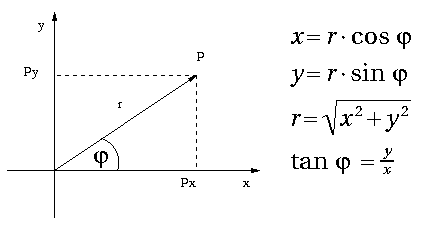
\includegraphics[scale=0.5]{img/Koordinatentransformation.png}
    \caption{Zusammenhänge Kartesische Koordinaten / Polarkoordinaten}
\end{figure}

Übertragen auf die Fourierreihen entspricht in der Grafik:
\begin{itemize}
    \item $a_k$ = $x$ (Sinus-Kosinus-Form)
    \item $b_k$ = $y$ (Sinus-Kosinus-Form)
    \item $A_k$ = $r$ (Spektralform)
    \item $\phi_k$ = $\phi$ (Spektralform)
\end{itemize}

Um den Winkel $\varphi$ im Interval $(-\pi, \pi]$ zu berechnen, gibt es mehrere
Möglichkeiten. Mithilfe des Arkustangens:
$$\varphi = \begin{cases}
    \arctan\frac{y}{x} & \mathrm{f\ddot ur}\ x > 0\\
    \arctan\frac{y}{x} + \pi & \mathrm{f\ddot ur}\ x < 0,\ y \geq 0\\
    \arctan\frac{y}{x} - \pi & \mathrm{f\ddot ur}\ x < 0,\ y < 0\\
    +\pi/2 & \mathrm{f\ddot ur}\ x = 0,\ y > 0\\
    -\pi/2 & \mathrm{f\ddot ur}\ x = 0,\ y < 0\\
\end{cases}$$

Falls man den Radius $r$ bzw. $A$ schon weiss, kann man auch den Arkuskosinus
verwenden:
$$\varphi = \begin{cases}
    +\arccos\frac{x}{r} & \mathrm{f\ddot ur}\ y\geq 0\\
    -\arccos\frac{x}{r} & \mathrm{f\ddot ur}\ y<0
\end{cases}$$


\subsection{Fourierreihen}

Die Funktion
$$f := t \mapsto a_0 + \sum_{k=1}^{\infty} \left[a_k \cos(k\omega_1t) + b_k
    \sin(k\omega_1t)\right]$$
$$= t \mapsto A_0 + \sum_{k=1}^{\infty} A_k \cos(k\omega_1 t - \varphi_k)$$
heisst die \emph{Fourierreihe} von $s$.


\subsection{Kriterium von Dirichlet}

Sei $s$ ein mit $T$ periodisches Signal, das innerhalb einer Periode aus
endlich vielen stetigen Stücken zusammengesetzt ist. Dann konvergieren die
Werte der Fourierreihe $f$ und zwar
\begin{itemize}
    \item an Stellen $t$, an denen das Signal stetig ist, gegen den Signalwert
    $$f(t) = s(t)$$
    \item an Stellen $t$, an denen das Signal nicht stetig ist, gegen den
    Mittelwert der beiden einseitigen Grenzwerte
    $$f(t) = \frac{\lim\limits_{\tau \mapsto t-}(f(\tau)) + \lim\limits_{\tau
        \mapsto t+}(f(\tau))}{2}$$
\end{itemize}


\subsection{Fourierreihen gerader und ungerader Signale}

Ein gerades, mit der Periode $T$ periodisches Signal $g$ besitzt eine reine
Kosinusreihe
$$f_g := t \mapsto a_0 + \sum_{k=1}^{\infty} \left[ a_k \cos(k\omega_1t)\right]
    \textrm{ mit } \omega_1 = \frac{2\pi}{T}$$
wobei
$$a_k = \frac{4}{T} \int\limits_0^{T/2} g(t) \cos(k\omega_1t) dt$$
gilt.

Ein ungerades, mit der Periode $T$ periodisches Signal $u$ besitzt eine reine
Sinusreihe
$$f_u := t \mapsto \sum_{k=1}^{\infty} \left[ b_k \sin(k\omega_1t)\right]
    \textrm{ mit } \omega_1 = \frac{2\pi}{T}$$
wobei
$$b_k = \frac{4}{T} \int\limits_0^{T/2} u(t) \sin(k\omega_1t) dt$$
gilt.


\subsection{Linearität der Fourierkoeffizienten}

$s_1$ und $s_2$ seien zwei Signale mit derselben Periode $T$. Die Konstanten
ihrer Fourierreihen seien $a_{1,0}$ beziehungsweise $a_{2,0}$ und die
Koeffizienten $a_{1,k}$, $b_{1,k}$ beziehungsweise $a_{2,k}$, $b_{2,k}$.

Dann ist die Summe beiden Signale
$$s = s_1 + s_2$$
periodisch mit derselben Periode und für die Konstante $a_0$, sowie die
Koeffizienten $a_k$ und $b_k$ ihrer Fourierreihe gelten folgende Beziehungen:
$$a_0 = a_{1,0} + a_{2,0}$$
$$a_k = a_{1,k} + a_{2,k}$$
$$b_0 = b_{1,k} + b_{2,k}$$
Ist ferner $c$ eine Konstante, so hat auch das Signal
$$\tilde{s} = c \cdot s$$
dieselbe Periode $T$, und die Konstante und Koeffizienten der
Fourierentwicklung sind
$$\tilde{a_0} = c \cdot a_0$$
$$\tilde{a_k} = c \cdot a_k$$
$$\tilde{b_x} = c \cdot b_k$$


\subsection{Spiegelung des Signalgraphen an der Ordinatenachse (Zeitumkehr)}

Das Signal $s$ sei periodisch mit der Periode $T$ und seine Fourierreihe sei
$$f:= t \mapsto a_0 + \sum_{k=1}^{\infty} \left[a_k\cos(k\omega_1t)
    + b_k\sin(k\omega_1t)\right]$$
$$= t \mapsto A_0 + \sum_{k=1}^{\infty} A_k \cos(k\omega_1t - \phi_k)
    \textrm{ mit } \omega_1 = \frac{2\pi}{T}$$
Dann hat das Signal
$$\tilde{s} := t \mapsto s(-t)$$
die Fourierreihe
$$\tilde{f} = t \mapsto a_0 + \sum_{k=1}^{\infty} \left[a_k \cos(k\omega_1t)
    - b_k\sin(k\omega_1t)\right]$$
$$= t \mapsto A_0 + \sum_{k=1}^{\infty} A_k\cos(k\omega_1t + \phi_k)$$
\textbf{Merke:} Durch die Spiegelung an der Ordinatenachse ändern die
Koeffizienten der Sinusglieder und die Phasen das Vorzeichen, während alle
anderen Bestimmungstücke unverändert bleiben.


\subsection{Zeitskalierung}

Das Signal $s$ sei periodisch mit der Periode $T$ und seine Fourierreihe sei
$$f:= t \mapsto a_0 + \sum_{k=1}^{\infty} \left[a_k\cos(k\omega_1t)
    + b_k\sin(k\omega_1t)\right]$$
$$= t \mapsto A_0 + \sum_{k=1}^{\infty} A_k \cos(k\omega_1t - \phi_k)
    \textrm{ mit } \omega_1 = \frac{2\pi}{T}$$
Dann hat das Signal
$$\tilde{s} := t \mapsto s(ct) \textrm{ für } c > 0$$
die Fourierreihe
$$\tilde{f} = t \mapsto a_0 + \sum_{k=1}^{\infty} \left[a_k \cos(k\omega_2t)
    + b_k\sin(k\omega_2t)\right]$$
$$= t \mapsto A_0 + \sum_{k=1}^{\infty} A_k\cos(k\omega_2t - \phi_k)$$
wobei
$$\omega_2 = c\omega_1$$
ist.\\\\
\textbf{Merke:} Durch die zeitliche Skalierung ändert einzige die
Grundkreisfrequenz, während die Fourierkoeffizienten, die Amplituden und die
Phasen unverändert bleiben.


\subsection{Zeitverschiebung}

Das Signal $s$ sei periodisch mit der Periode $T$ und seine Fourierreihe sei
$$f:= t \mapsto a_0 + \sum_{k=1}^{\infty} \left[a_k\cos(k\omega_1t)
    + b_k\sin(k\omega_1t)\right]$$
$$= t \mapsto A_0 + \sum_{k=1}^{\infty} A_k \cos(k\omega_1t - \phi_k)
    \textrm{ mit } \omega_1 = \frac{2\pi}{T}$$
Dann hat das Signal
$$\tilde{s} := t \mapsto s(t-\tau)$$
die Fourierreihe
$$t \mapsto \widetilde{a_0} + \sum_{k=1}^{\infty} \left[\widetilde{a_k}
    \cos(k\omega_1t) + \widetilde{b_k}\sin(k\omega_1t)\right]$$
$$= t \mapsto \widetilde{A_0} + \sum_{k=1}^{\infty}
    \widetilde{A_k}\cos(k\omega_1t - \widetilde{\phi_k})$$
mit
$$\widetilde{a_0} = a_0$$
$$\widetilde{a_k} = a_k\cos(k\gamma) - b_k\sin(k\gamma)$$
$$\widetilde{b_k} = a_k\sin(k\gamma) + b_k\cos(k\gamma)$$
$$\widetilde{A_k} = A_k$$
$$\widetilde{\phi_k} = \phi_k + k\gamma$$
wobei
$$\gamma = \frac{\tau}{T} \times 2\pi$$
ist.\\\\
\textbf{Merke:} Bei einer zeitlichen Verzögerung des Signals ändern nur die
Phasen, während die Konstante und die Amplituden gleich bleiben.


\subsection{Fourierintegral}

$s$ sei ein Signal, welches absolut integrierbar ist, das heisst, für welches
das Integral
$$\int\limits_{-\infty}^{\infty} |s(t)|dt$$
existiert. Dann existieren auch die beiden Integrale
$$a(\omega) = \frac{1}{\pi} \int\limits_{-\infty}^{\infty} s(t)
    \cos(\omega t)dt$$
$$b(\omega) = \frac{1}{\pi} \int\limits_{-\infty}^{\infty} s(t)
    \sin(\omega t)dt$$
Die Funktion
$$f := t \mapsto \int\limits_0^{\infty} \left[ a(\omega) \cos(\omega t)
    + b(\omega) \sin(\omega t)\right]dw$$
$$=t \mapsto \int\limits_0^{\infty} \left[A(\omega) \cos(\omega t
    - \phi (\omega))\right]dw$$
heisst die \emph{Fouriertransformierte} oder das \emph{Fourierintegral} von
$s$. Die erste Form heisst \emph{Sinus-Kosinus-Form}, die zweite
\emph{Spektralform} oder \emph{Amplituden-Phasen-Form}. Wenn
$(a(\omega), b(\omega))$ die kartesischen Koordinaten eine Punktes in der Ebene
sind, dann sind $(A(\omega), \phi(\omega))$ die Polarkoordinaten dieses Punktes.


\subsection{Satz von Dirichlet}

Mit den Bezeichnungen der obigen Definition gilt:
\begin{itemize}
\item Wenn $s$ an der Stelle $t$ stetig ist, so ist $f(t) = s(t)$
\item Wenn nicht, so ist $\displaystyle f(t) = \frac{1}{2} \left(\lim_{\tau
    \mapsto t-}(s(\tau)) + \lim_{\tau \mapsto t+}(s(\tau))\right)$
\end{itemize}


\section{Differenzialgleichungen}


\subsection{Die Differenzialgleichung}

Eine Gleichung zwischen einer Funktion und ihren Ableitungsfunktionen heisst
\emph{Differenzialgleichung}. Die höchste vorkommende Ableitung heisst die
\emph{Ordnung} der Differenzialgleichung. Eine Differenzialgleichung hat in der
Regel unendlich viele Lösungen. Die Lösungsmenge nennt man aus historischen
Gründen auch die \emph{allgemeine Lösung} und eine einzelne Lösung eine
\emph{spezielle Lösung}.  Zusätzliche Bedingungen, welche dazu dienen, aus der
allgemeinen Lösung eine spezielle auszusondern, heissen \emph{Randbedingungen}
oder \emph{Anfangsbedingungen} (wenn das Argument die Zeit darstellt). Eine
Differenzialgleichung mit Randbedingungen wird auch als \emph{Randwertproblem}
oder \emph{Anfangswertproblem} bezeichnet.

\textbf{Merke:} Angewandte Probleme, bei denen eine ganze Funktion gesucht ist,
führen auf Differenzialgleichungen.


\subsubsection{Explizite Differenzialgleichungen}

Eine Differenzialgleichung, in der die höchste Ableitung isoliert auf einer
Seite des Gleichheitszeichens steht, heisst \emph{explizit}. Eine explizite
Differenzialgleichung für die Funktion $f$ hat also die Gestalt
$$f^{(n)}(x) = G\left(x,f(x),f'(x),\dotsc,f^{(n-1)}(x)\right)$$
im Spezialfall einer Differenzialgleichung 1. Ordnung somit
$$f'(x) = G(x,f(x))$$
In diesem Fall ist die rechte Seite ist also nur vom Argument $x$ und vom Wert
$fx$ der gesuchten Funktion abhängig; die Ableitung hingegen kommt rechts nicht
vor.


\subsubsection{Separierbare Differenzialgleichung}

Eine Differenzialgleichung für die Funktion $f$ heisst \emph{separierbar}, wenn
sie auf die Form
$$f'(x) = \frac{g(x)}{h(f(x))}$$
gebracht werden kann.


\subsubsection{Lineare Differenzialgleichung}

Eine Differenzialgleichung für die Funktion $f$ der Form
$$a_0 f(x) + a_1 f'(x) + a_2 f''(x) + \dotsb + a_n f^{(n)}(x) = s(x)$$
oder
$$\sum\limits_{k=0}^n a_k f^{(k)}(x) = s(x)$$
wobei die $a_k$ gegebene Konstanten und $s$ eine vorgegebene Funktion ist,
heisst \emph{lineare Differenzialgleichung} mit konstanten Koeffizienten. Die
$a_k$ heissen die \emph{Koeffizienten}, $s$ die \emph{Störfunktion}.

Wenn die Störfunktion die Nullfunktion ist, heisst die Differenzialgleichung
\emph{homogen}, andernfalls \emph{inhomogen}.


\subsection{Methode von Euler}

Gegeben sei eine explizite Differenzialgleichung 1. Ordnung für die Funktion $f$
$$f'(x) = G(x, y) = G(x,f(x))$$
und ein Punkt $P_n = (x_n,y_n)$ des Graphen einer speziellen Lösung.

Der Punkt $P_{n+1} = (x_{n+1}, y_{n+1})$ wird wie folgt bestimmt:\\
Man wählt ein $\Delta{x}$ mit kleinem Betrag und berechnet
$$x_{n+1} = x_n + \Delta x$$
$$y_{n+1} = y_n + s_n\Delta x$$
mit
$$s_n = G(x_n,y_n)$$


\subsection{Verfahren von Runge-Kutta}

Gegeben sei eine explizite Differenzialgleichung 1. Ordnung für die Funktion $f$
$$f'(x) = G(x, f(x))$$
und ein Punkt $P_n = (x_n, y_n)$ des Graphen einer speziellen Lösung.

Der Punkt $P_{n+1} = (x_{n+1},y_{n+1})$ wird wie folgt bestimmt:\\
Man wählt ein $\Delta{x}$ mit kleinem Betrag. Die Abszisse von $P_{n+1}$ ist
$$x_{n+1} = x_n + \Delta x$$
Die Ordinate ist
$$y_{n+1} = y_n + s\Delta x$$
mit
$$s = \frac{s_1 + 2s_2 + 2s_3 + s_4}{6}$$
wobei
\begin{enumerate}
    \item $\displaystyle s_1 = G(x_n, y_n)$
    \item $\displaystyle s_2 = G\left(x_n + \frac{\Delta{x}}{2}, y_n + s_1
        \frac{\Delta x}{2}\right)$
    \item $\displaystyle s_3 = G\left(x_n + \frac{\Delta{x}}{2}, y_n + s_2
        \frac{\Delta x}{2}\right)$
    \item $\displaystyle s_4 = G(x_n+\Delta x, y_n+s_3\Delta x)$
\end{enumerate}


\subsection{Linearität der Lösungen homogener linearer Differenzialgleichungen}

\begin{enumerate}
    \item Wenn $f_1$ und $f_2$ Lösungen einer homogenen linearen
        Differenzialgleichung sind, so ist auch ihre Summe $f_1 + f_2$ eine
        Lösung.
    \item Ist ferner $f$ eine Lösung und $c$ eine Konstante, so ist auch das
        Produkt $c \cdot f$ eine Lösung.
\end{enumerate}

Man kann die beiden Gesetze auch so zusammenfassen:

Wenn $f_1$ und $f_2$ Lösungen einer homogenen linearen Differenzialgleichung
sind, so ist auch jede Linearkombination $c_1f_1 + c_2f_2$, wobei $c_1$ und
$c_2$ Konstanten sind, eine Lösung.


\subsection{Allgemeine Lösung homogener Linearer Differenzialgleichungen
    zweiter Ordnung}

Gegeben sei die homogene lineare Differenzialgleichung
$$c_2f''(x) + c_1f'(x) + c_0f(x) = 0$$
Um sie zu lösen, formuliert man zuerst ihre \emph{charakteristische Gleichung}.
$$c_2s^2 + c_1s + c_0 = 0$$
Nun sind drei Fälle zu unterscheiden:

\begin{itemize}
    \item Wenn die charakteristische Gleichung \textbf{zwei verschiedene}
        Lösungen $s_1$ und $s_2$ besitzt (die Diskriminante $b^2 - 4ac$ also
        positiv ist), so lautet die allgemeine Lösung der Differenzialgleichung
        $$f := x \mapsto Ae^{s_1 x} + Be^{s_2 x}$$
        mit frei wählbaren Konstanten $A$ und $B$.
    \item Wenn die charakteristische Gleichung \textbf{nur eine} Lösung $s_1$
        besitzt (die Diskriminante $b^2 - 4ac$ also Null ist), so lautet die
        allgemeine Lösung der Differenzialgleichung
        $$f := x \mapsto (Ax + B)e^{sx}$$
        mit frei wählbaren Konstanten $A$ und $B$.
    \item Wenn die charakteristische Gleichung keine Lösung hat (die
        Diskriminante $b^2 - 4ac$ also negativ ist) so lautet die allgemeine
        Lösung der Differenzialgleichung
        $$f := x \mapsto e^{rx}\left(A \cos(\omega x)
            + B \sin(\omega x)\right)$$
        mit frei wählbarem $A$ und $B$, respektive in der Amplituden-Phasen-Form
        $$f := x \mapsto Ce^{rx} \cos(\omega x - \phi)$$
        mit frei wählbarem $C$ und $\phi$.

        Um die Parameter $r$ und $\omega$ zu bestimmen, bringt man die rechte
        Seite der Lösungsformel für die charakteristische Gleichung auf die Form
        $$s = a \pm \sqrt{b}$$
        Dann ist
        $$r = a \textrm{ und } \omega = \sqrt{-b}$$
\end{itemize}


\subsection{Inhomogene lineare Differenzialgleichungen}

Die allgemeine Lösung einer inhomogenen linearen Differenzialgleichung für $f$
$$\sum_{k=0}^n a_k f^{(k)}(x) = s(x)$$
ist die Summe einer partikulären Lösung und der allgemeinen Lösungen der
zugehörigen homogenen Gleichung
$$\sum_{k=0}^n a_k f^{(k)}(x) = 0$$


\end{document}
